\section{服务器相关}
% \lipsum[1-2]
\subsection{服务器基础架构}
\begin{figure}[H]
	\centering
	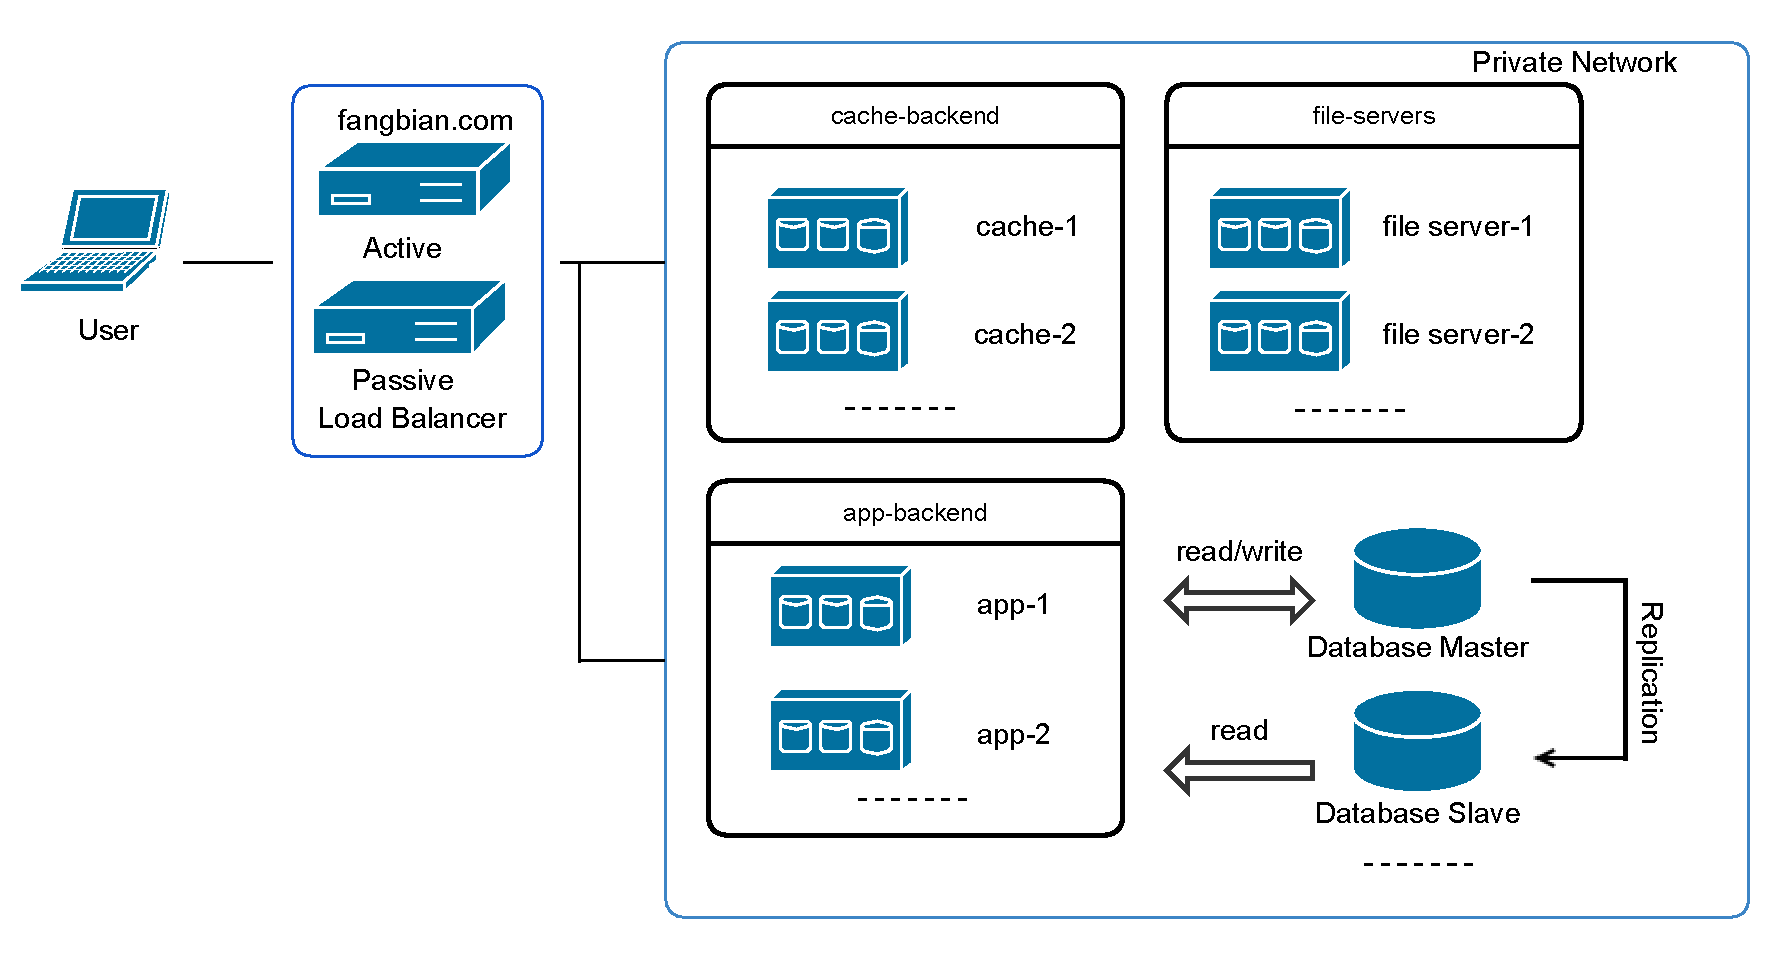
\includegraphics[width=1.0\textwidth]{graphics/diagramsvg.pdf}
	\caption{服务器3-Tier基础设置}
	\label{fig:hs}
\end{figure}

\begin{enumerate}[label=(\alph*)]
   \item 请求动态内容。
     \begin{enumerate}[label=(\arabic*)]
       \item 用户向fangbian.com(load balancer)请求
       \item load balancer向后端应用服务器(app-backend)发出请求
       \item app-backend读取数据库并向load balancer返回内容
       \item load balancer向用户返回请求内容
     \end{enumerate}

   \item 请求静态内容。
     \begin{enumerate}[label=(\arabic*)]
       \item 用户向fangbian.com(load balancer)请求
       \item load balancer从cache-backend检查请求内容是cache-hit还是cache-miss
       \item 如果是cache-hit,向load balancer返回请求内容且跳至第7步;如果是cache-miss,则通过load balancer将请求转到app-backend
       \item app-backend从数据库读取并返回内容到load balancer
       \item load balancer将收到的内容传递到cache-backend 
       \item cache-backend缓存内容然后向load balancer返回内容
       \item load balancer向用户返回请求内容
     \end{enumerate}
\end{enumerate}
\par 提示:设置active/passive负载均衡对(需要虚拟/浮动IP(LVS))可以应对负载均衡失效的问题。例如HAProxy,Nginx等。

\subsection{整体网络架构}
\begin{figure}[H]
	\centering
	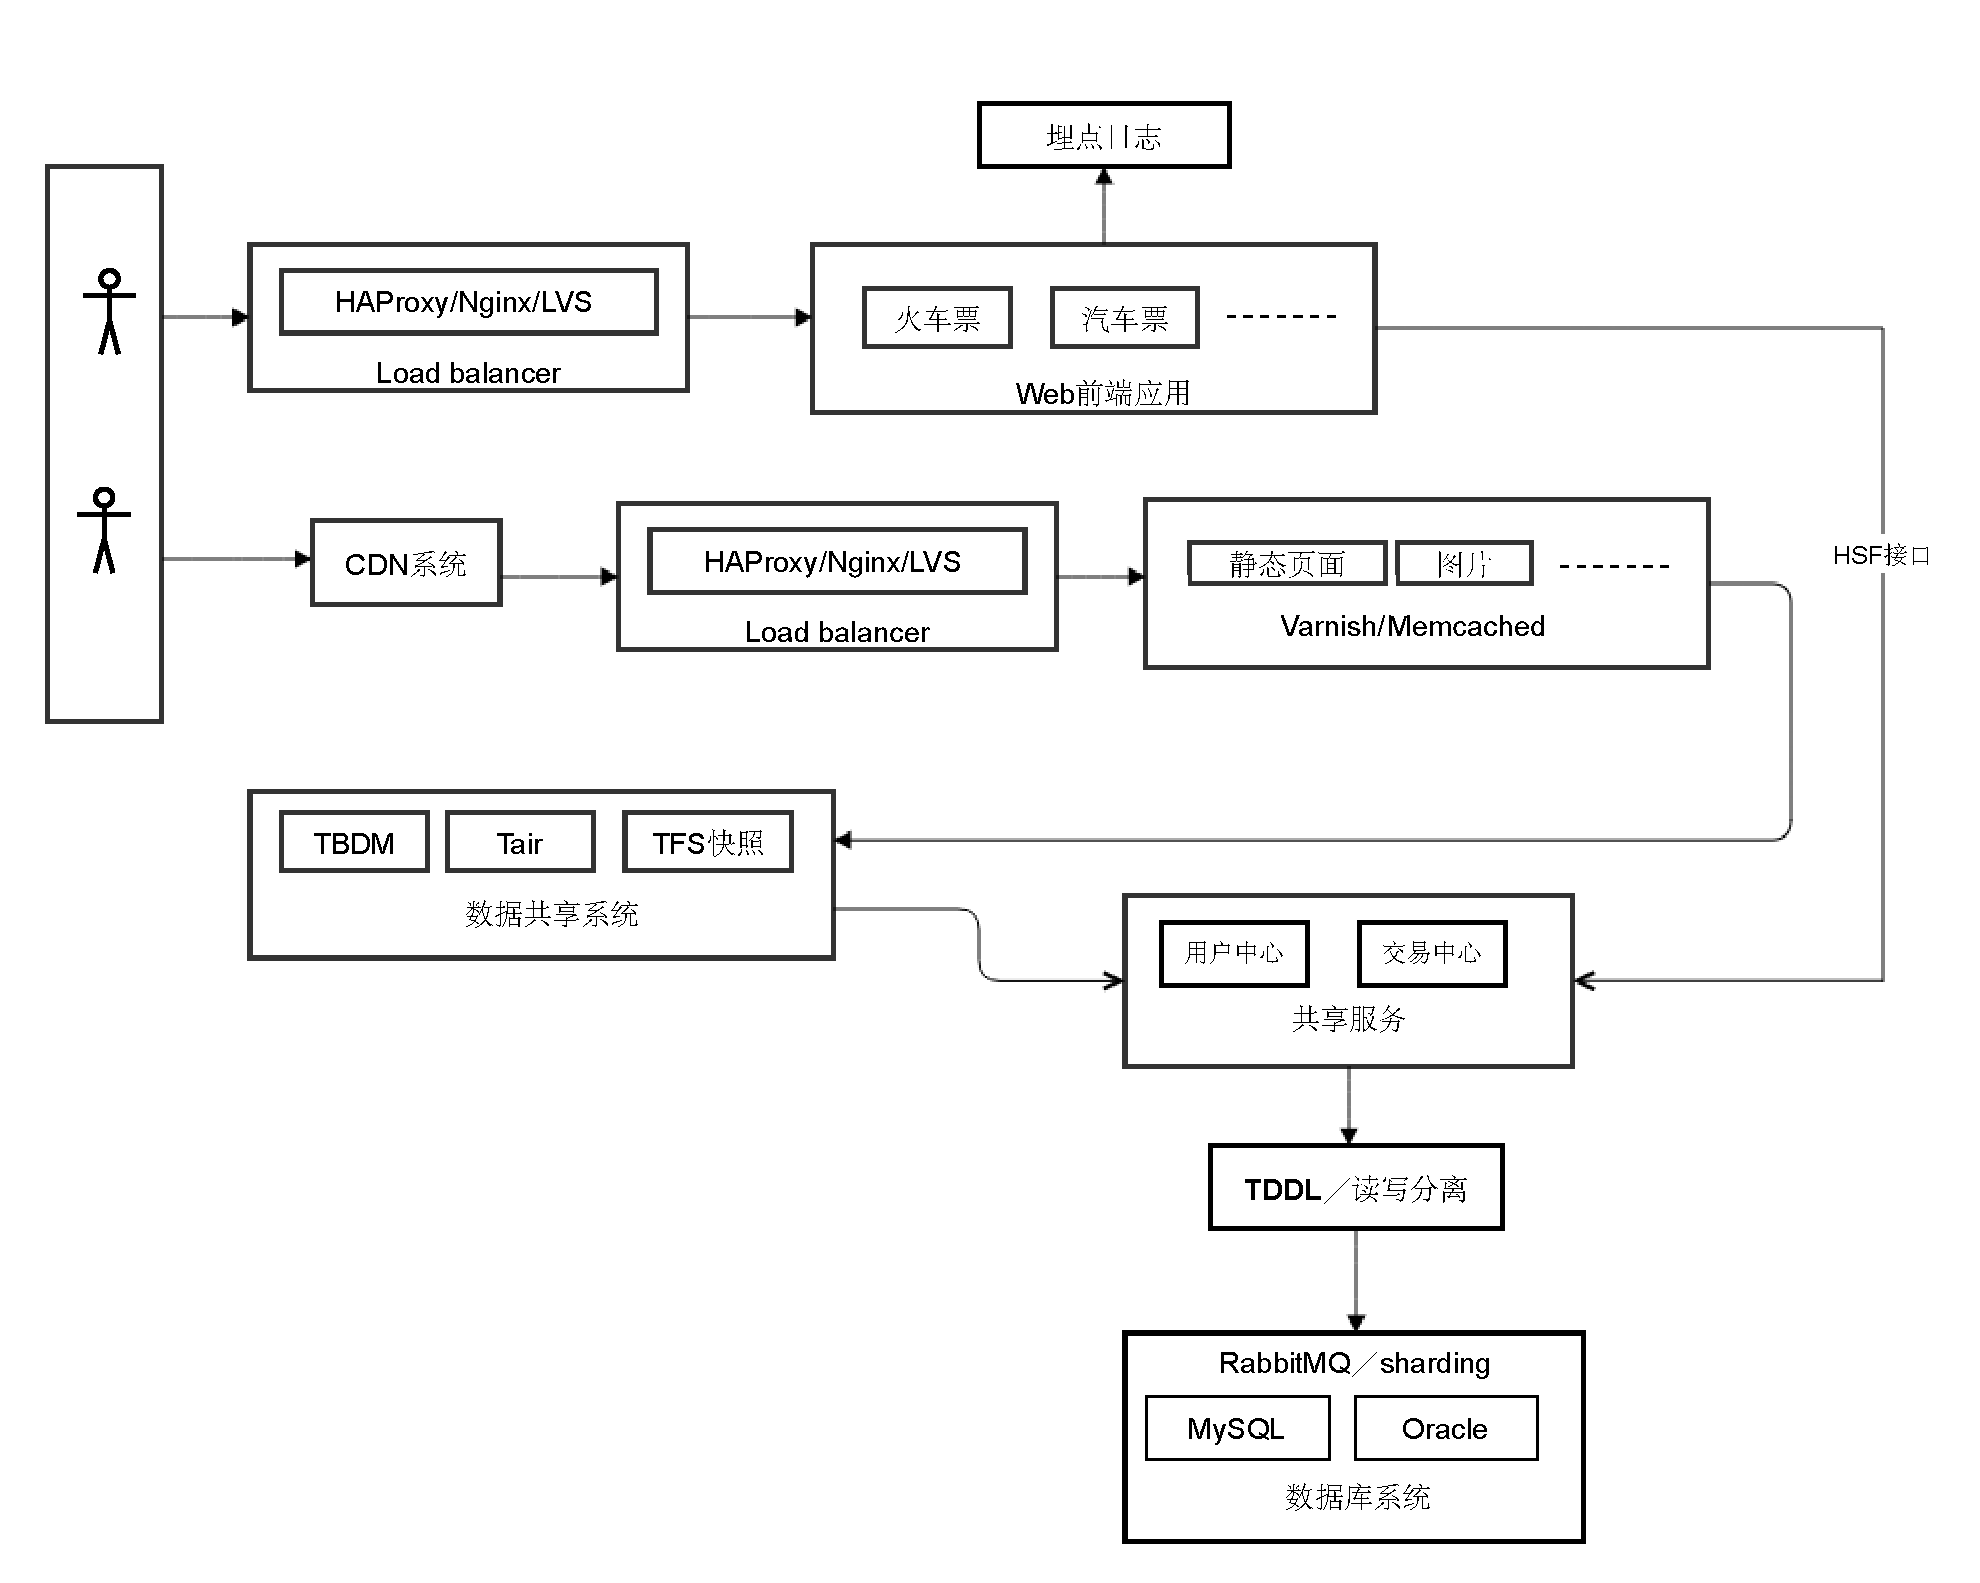
\includegraphics[width=1.0\textwidth]{graphics/tech.pdf}
	\caption{整体网络架构图}
	\label{fig:tech}
\end{figure}


\subsection{分布式架构的服务相关内容}
\begin{figure}[H]
	\centering
	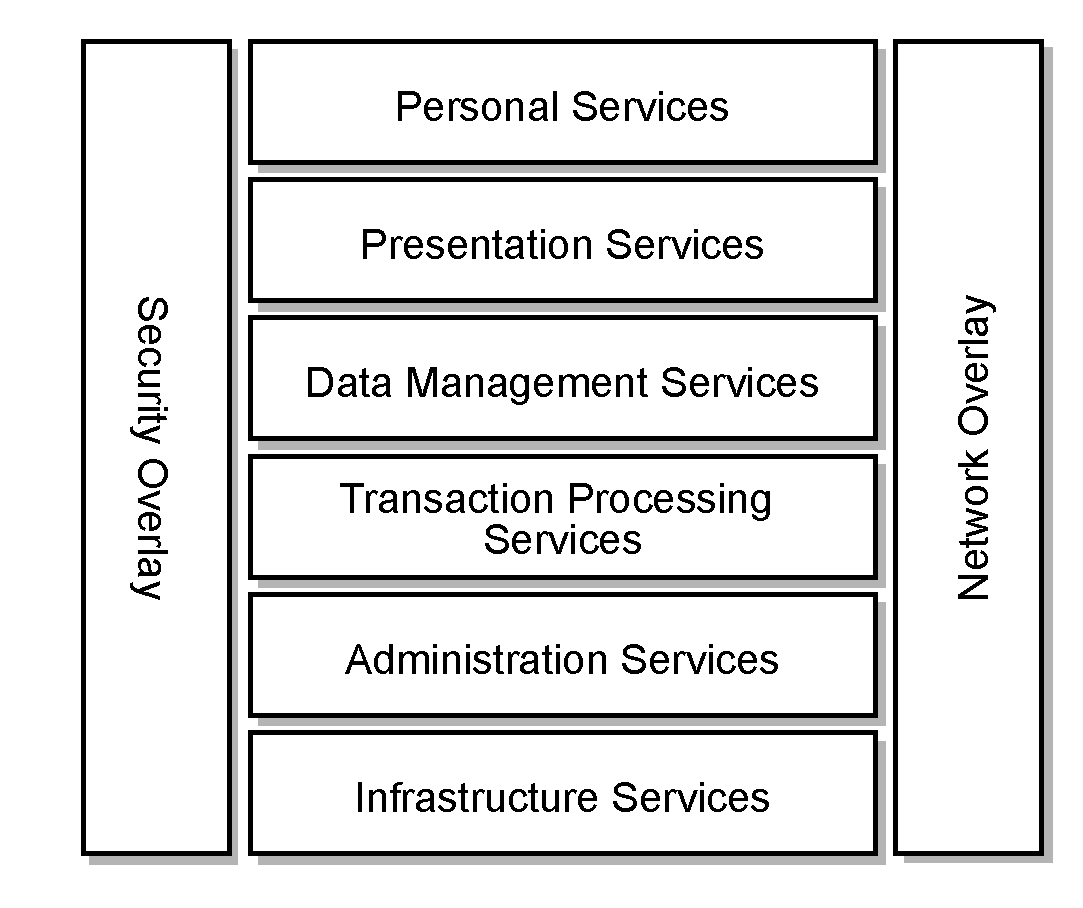
\includegraphics[width=0.7\textwidth]{graphics/architecture.pdf}
	\caption{分布式架构}
	\label{fig:architecture}
\end{figure}

\subsubsection{个人服务}
\begin{enumerate}
   \item 任何基于浏览器的应用。
   \item 建议:
       \begin{enumerate}[label=(\arabic*)]
       \item 坚持标准
       \item 避免使用只针对特定浏览器的特性
       \item 尽量简化逻辑判断
       \item 使用后端语言实现复杂逻辑
     \end{enumerate}
\end{enumerate}

\subsubsection{展现服务}
\begin{enumerate}
   \item 动态内容分发。
   \item 格式化与数据读取。
   \item web组件(例如Portlets)
   \item 建议:
       \begin{enumerate}[label=(\arabic*)]
       \item 数据读取和格式化分离
       \item 业务规则和显示逻辑不能混在一起
       \item 可以参考MVC
     \end{enumerate}
\end{enumerate}

\subsubsection{数据处理服务}
\begin{enumerate}
   \item 搜索。
   \item 分类。
   \item 内容聚合。
   \item 成员协作。
   \item 分配。
   \item 建议:
       \begin{enumerate}[label=(\arabic*)]
       \item 鉴定用户类型;
       \item 关注特定用户类型的目标;
       \item 考虑性能;
       \item 可以参考Chain of Responsibility Patterns和Presentation-Abstraction-Control.
     \end{enumerate}
\end{enumerate}

\subsubsection{交易处理服务}
\begin{enumerate}
   \item 交易管理。
   \item 元数据控制。
   \item 应用接口。
   \item 业务规则。
   \item 数据交换。
   \item 建议:
       \begin{enumerate}[label=(\arabic*)]
       \item 关注接口;
       \item 关注用户未完成的活动;
       \item 不要在业务规则上Hard coding;
       \item 参考observer,Adapter;
     \end{enumerate}
\end{enumerate}

\subsubsection{管理服务}
\begin{enumerate}
   \item LDAP.
   \item 系统管理。
   \item 状态管理。
   \item session管理。
   \item 用户控制。
   \item 规则定义。
   \item 建议:
       \begin{enumerate}[label=(\arabic*)]
       \item 定义策略;
       \item 控制系统状态;
       \item 预估增长;
       \item 参考Command 和 Microkernel;
     \end{enumerate}
\end{enumerate}

\subsubsection{基础设施服务}
\begin{enumerate}
   \item data access.
   \item 通信。
   \item 进程和线程管理。   
   \item 建议:
       \begin{enumerate}[label=(\arabic*)]      
       \item 参考Abstract Factory;
     \end{enumerate}
\end{enumerate}

\subsubsection{安全覆盖层}
\begin{enumerate}
   \item 硬件防火墙.
   \item 软件防火墙。
   \item SSL and WTLS。   
   \item 数据加密。   
   \item 建议:
       \begin{enumerate}[label=(\arabic*)]      
       \item 建立相关策略;
       \item 入侵监视;
       \item patch;
     \end{enumerate}
\end{enumerate}

\subsubsection{网络覆盖层}
\begin{enumerate}
   \item 路由,网关.
   \item 负载均衡。
   \item 建议:
       \begin{enumerate}[label=(\arabic*)]      
       \item 文档,标签,图表;
       \item 将各主要应用分开;
     \end{enumerate}
\end{enumerate}

\par 注:应对集群节点可能出现的故障,可以使用keepalived来解决。http://www.keepalived.org/
% \par 静态文件,用Varnish缓存
% \par 对数据库查询的数据,使用Memcached。
% \par 容灾:赛门铁克,爱数
% \par MySQL sharding 